\section{Case Study: 200 Nodes}
\subsection{Introduction}\label{subsec:case-study-200}
In this chapter we analyze the case at 200 nodes, as it is the quantity that is halfway between our configurations. At the end of the simulations we decide to calculate the average coverage percentage, summarized in this table.


\begin{table}[H]
\centering
\begin{tabular}{|c|c|c|c|c|c|}
\hline
 & \textbf{r=10} & \textbf{r=30} & \textbf{r=50} & \textbf{r=75} & \textbf{r=100} \\ \hline
\textbf{p=0.15} & 0,9073 & 1 & 1 & 1 & 1 \\ \hline
\textbf{p=0.3} & 0,8938 & 0,9992 & 0,9956 & 1 & 0,9992 \\ \hline
\textbf{p=0.5} & 0,7991 & 0,9942 & 0,9880 & 0,9889 & 0,9959 \\ \hline
\textbf{p=0.7} & 0,7105 & 0,9798 & 0,9645 & 0,9373 & 0,9903 \\ \hline
\textbf{p=0.85} & 0,5730 & 0,9421 & 0,9021 & 0,9183 & 0,9797 \\ \hline
\textbf{p=1} & 0,4755 & 0,8191 & 0,6712 & 0,7630 & 0,9673 \\ \hline
\end{tabular}
\caption{Mean coverage percentage}
\label{tab:mean-coverage-percentage}
\end{table}

The following table show the mean coverage time for each run.

\begin{table}[H]
\centering
\begin{tabular}{|c|c|c|c|c|c|}
\hline
 & \textbf{r=10} & \textbf{r=30} & \textbf{r=50} & \textbf{r=75} & \textbf{r=100} \\ \hline
\textbf{p=0.15} & 111,0152 & 45,1364 & 49,0455 & 47,6515 & 41,0152 \\ \hline
\textbf{p=0.3} & 61,8636 & 26,0152 & 29,5909 & 25,3182 & 18,2879 \\ \hline
\textbf{p=0.5} & 37,8333 & 20,5606 & 21,3182 & 16,7727 & 11,0455 \\ \hline
\textbf{p=0.7} & 28,0152 & 17,1970 & 15,6515 & 10,5303 & 7,0758 \\ \hline
\textbf{p=0.85} & 21,4091 & 13,6818 & 11,1061 & 7,2576 & 4,6515 \\ \hline
\textbf{p=1} & 16,8939 & 9,9242 & 3,8030 & 1,5 & 1,5 \\ \hline
\end{tabular}
\caption{Mean coverage time}
\label{tab:mean-coverage-time}
\end{table}


Since the means do not include any information on the variance of the data, we decide to plot a column graph showing the 90\% confidence interval for the average coverage values (Fig. \ref{fig:200-90CI}). Note that we chose to discard all runs that do not end with a coverage percentage above 95\% with a 90\% coverage. That's why in the following boxplot the runs with radius 10 are not shown.

\begin{figure}[h!]
\centering
\begin{subfigure}{.5\textwidth}
  \centering
  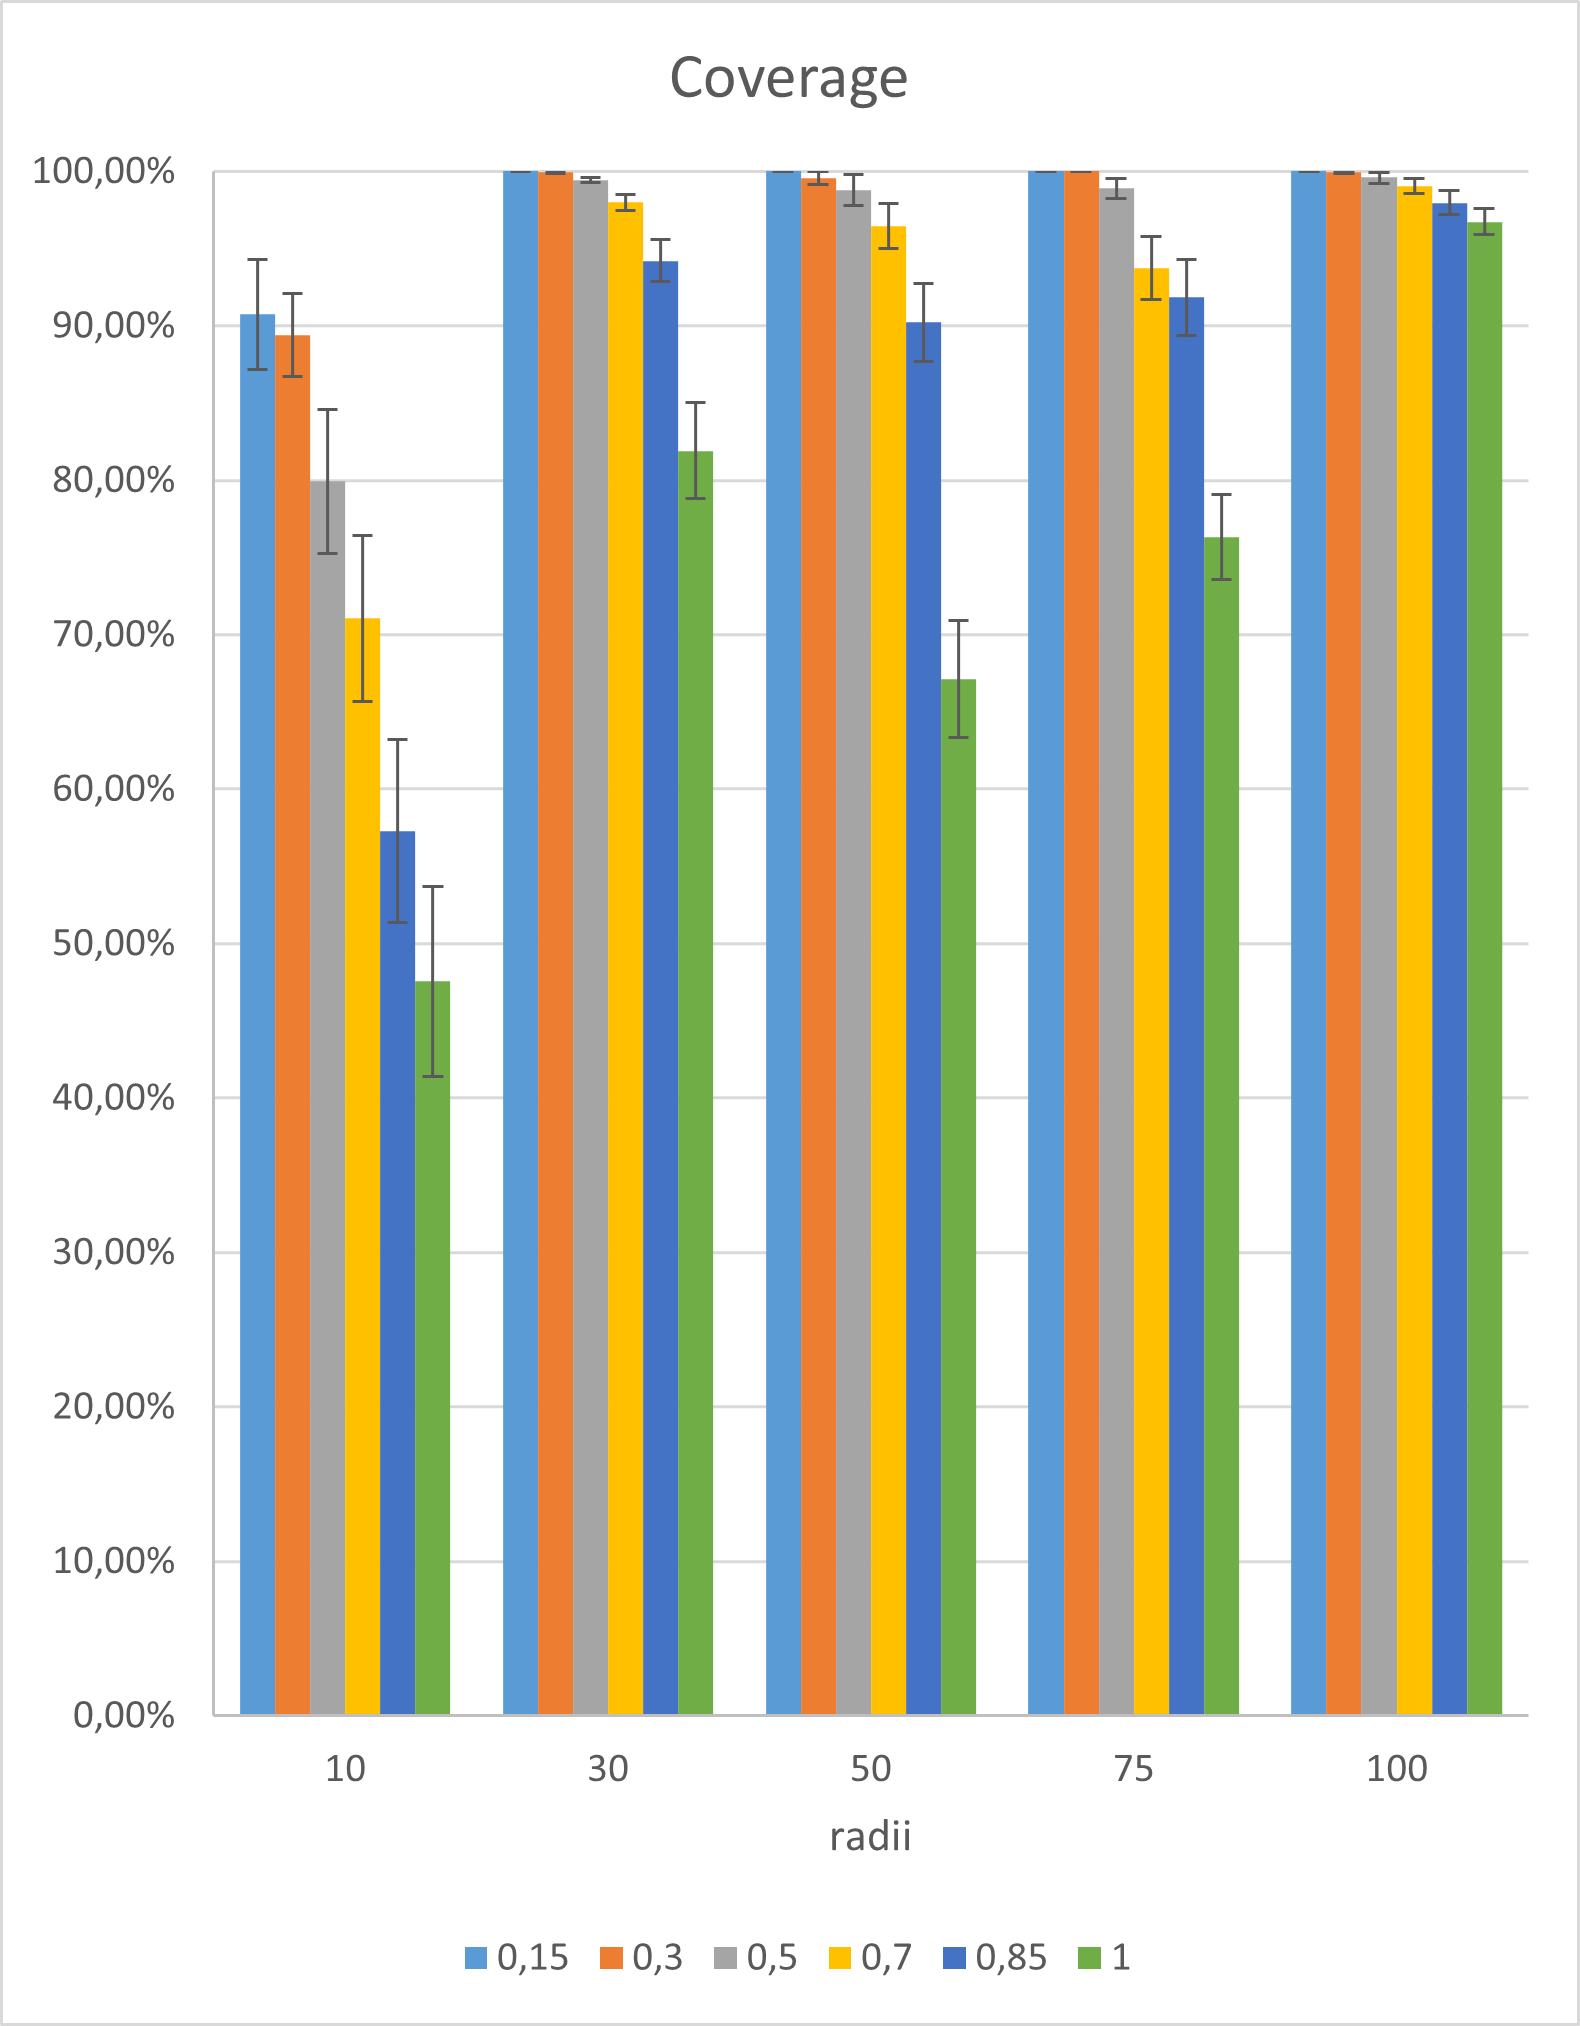
\includegraphics[width=1\linewidth]{./images/200coverageCI.png}
  \caption{Coverage percentage}
  \label{fig:CoveragePercentageCI}
\end{subfigure}%
\begin{subfigure}{.5\textwidth}
  \centering
  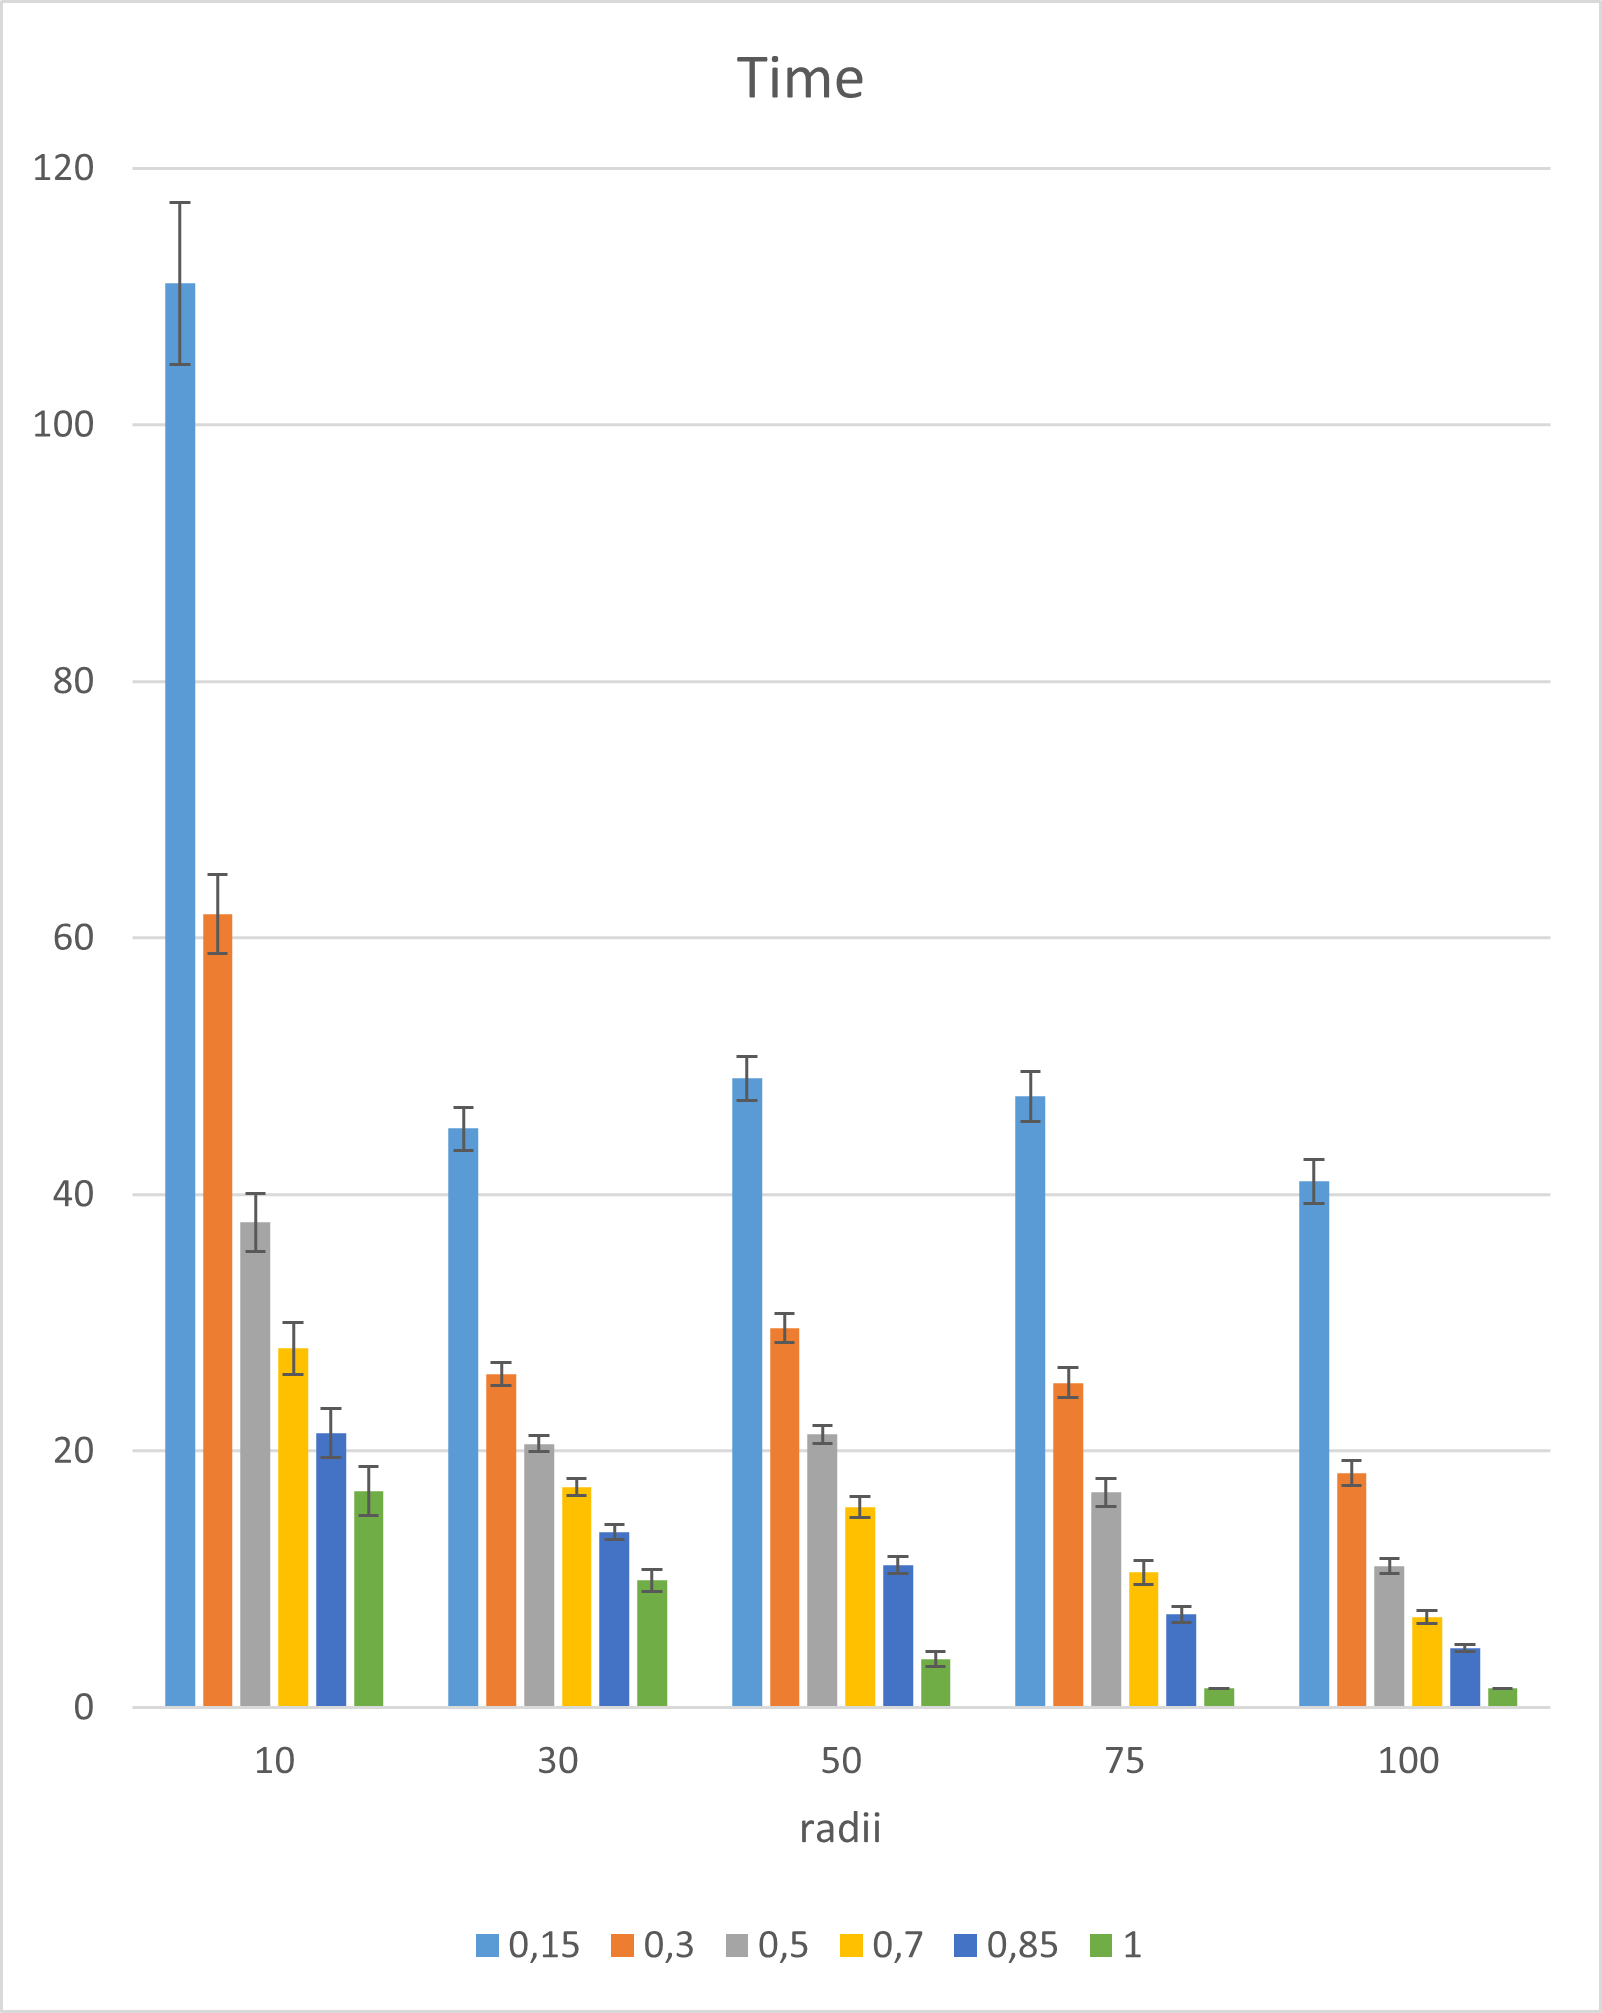
\includegraphics[width=1\linewidth]{./images/200endtimeCI.png}
  \caption{Coverage time}
  \label{fig:CoverageTimeCI}
\end{subfigure}
\caption{Column graph with 90\% CI}
\label{fig:200-90CI}
\end{figure}


\iffalse

\begin{figure}[h!]
    \centering
    \subfloat[\centering Coverage percentage]{{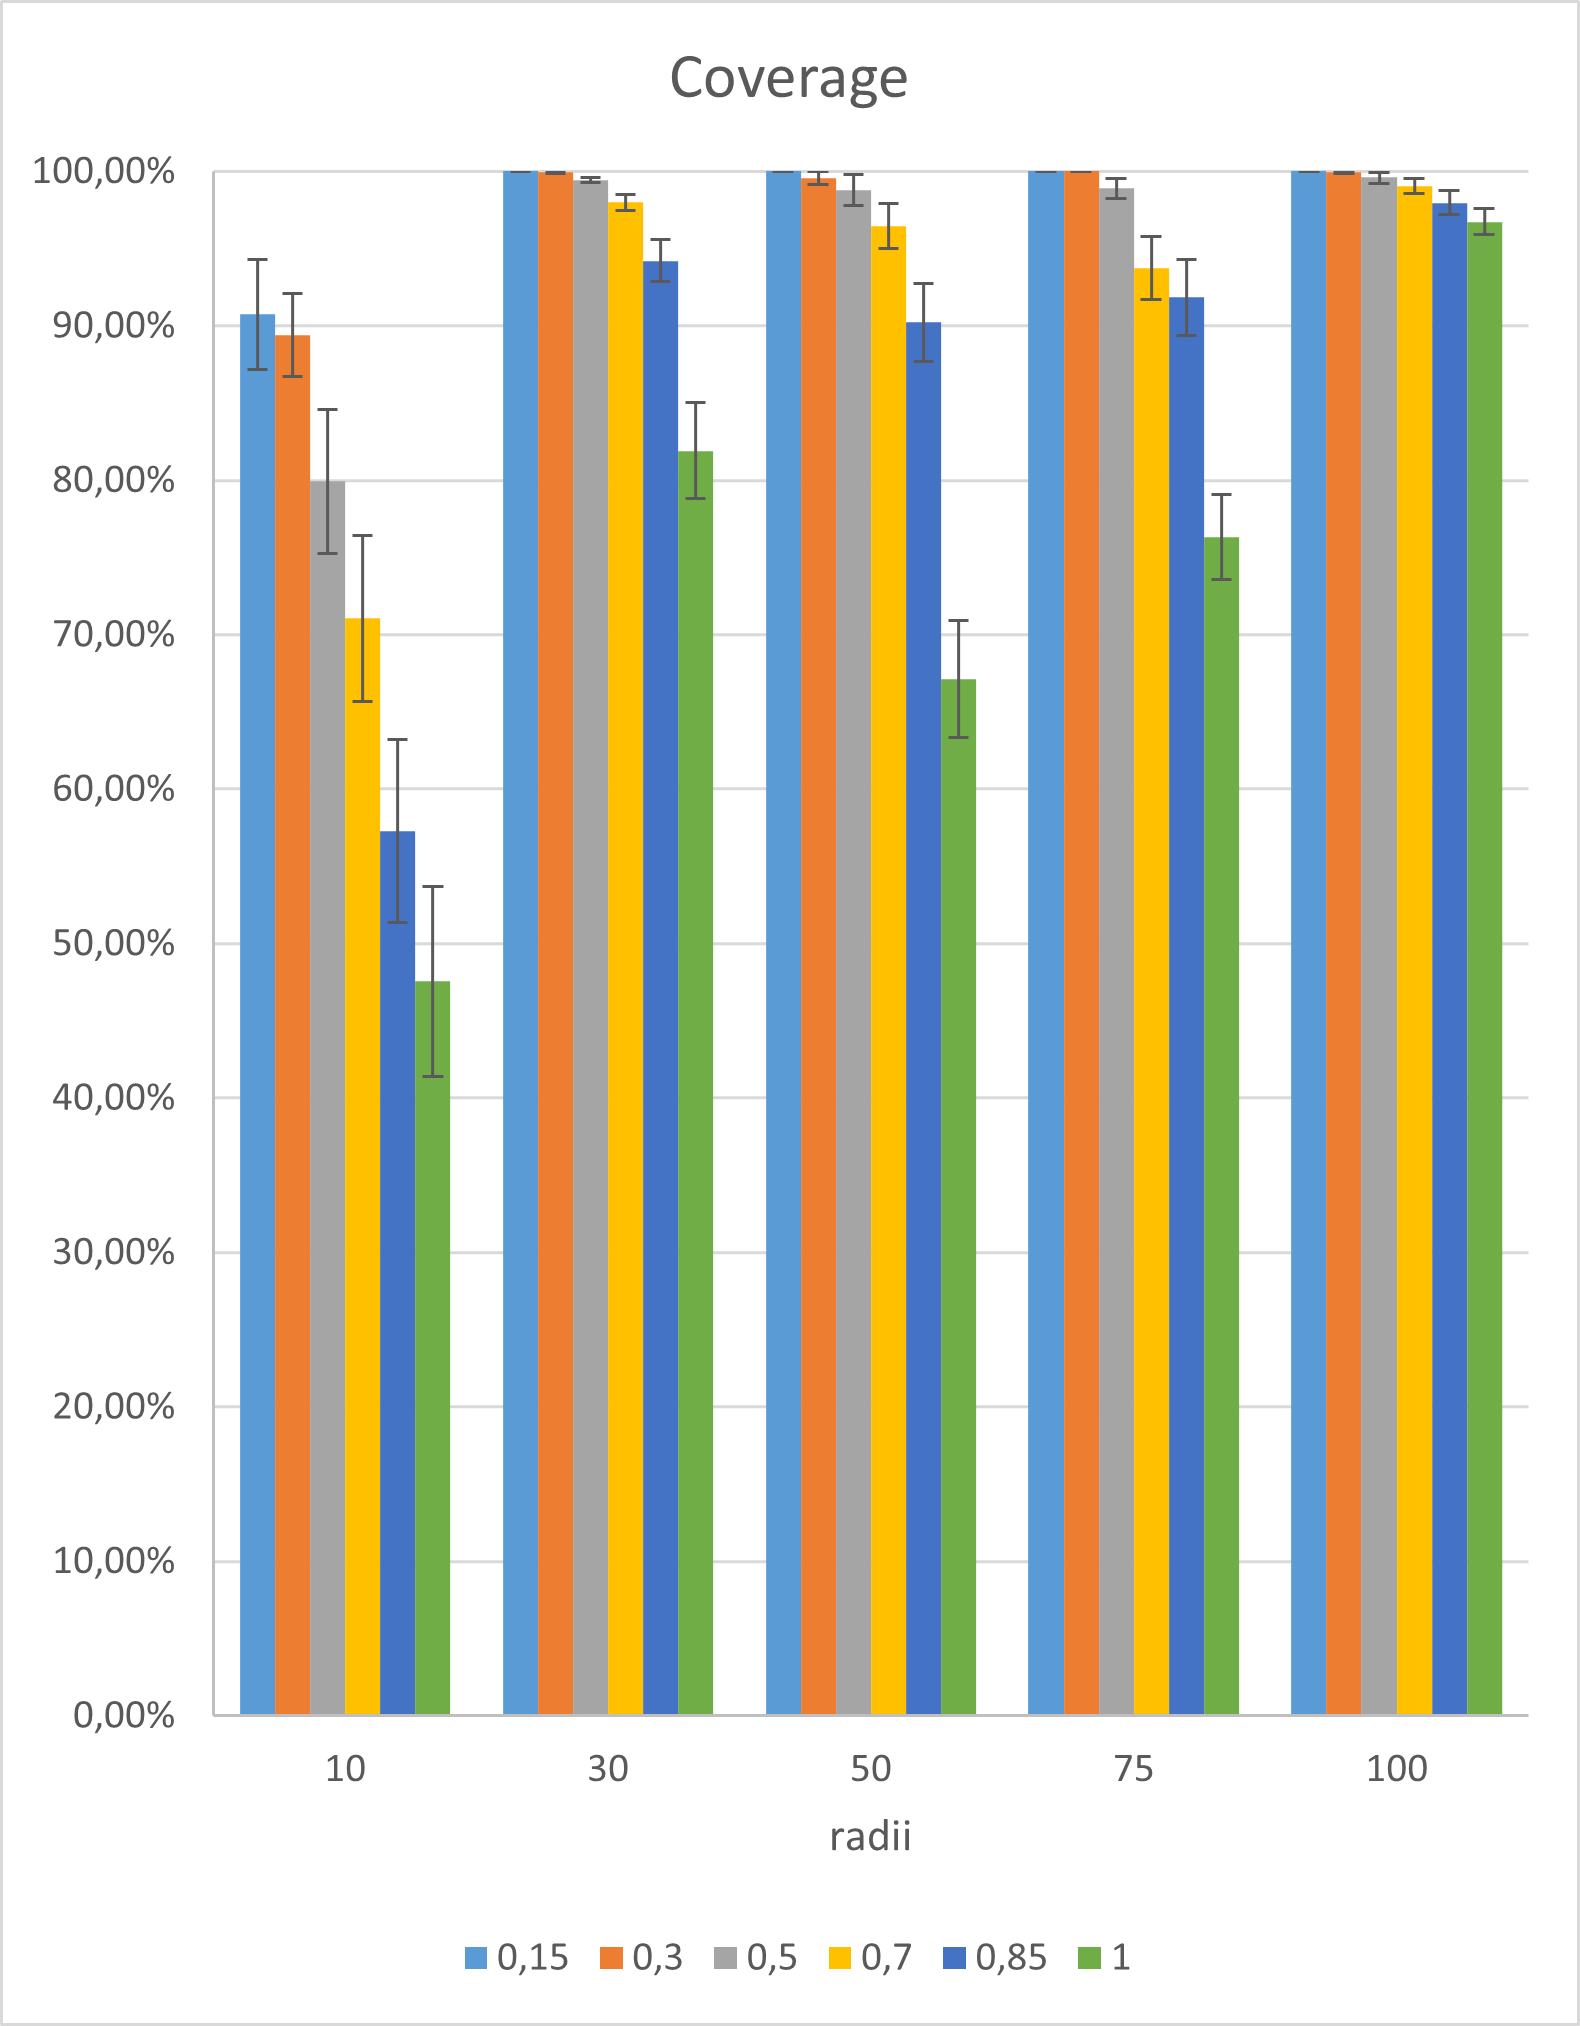
\includegraphics[width= 8cm]{./images/200coverageCI.png}}}
    \qquad
    \subfloat[\centering Coverage time]{{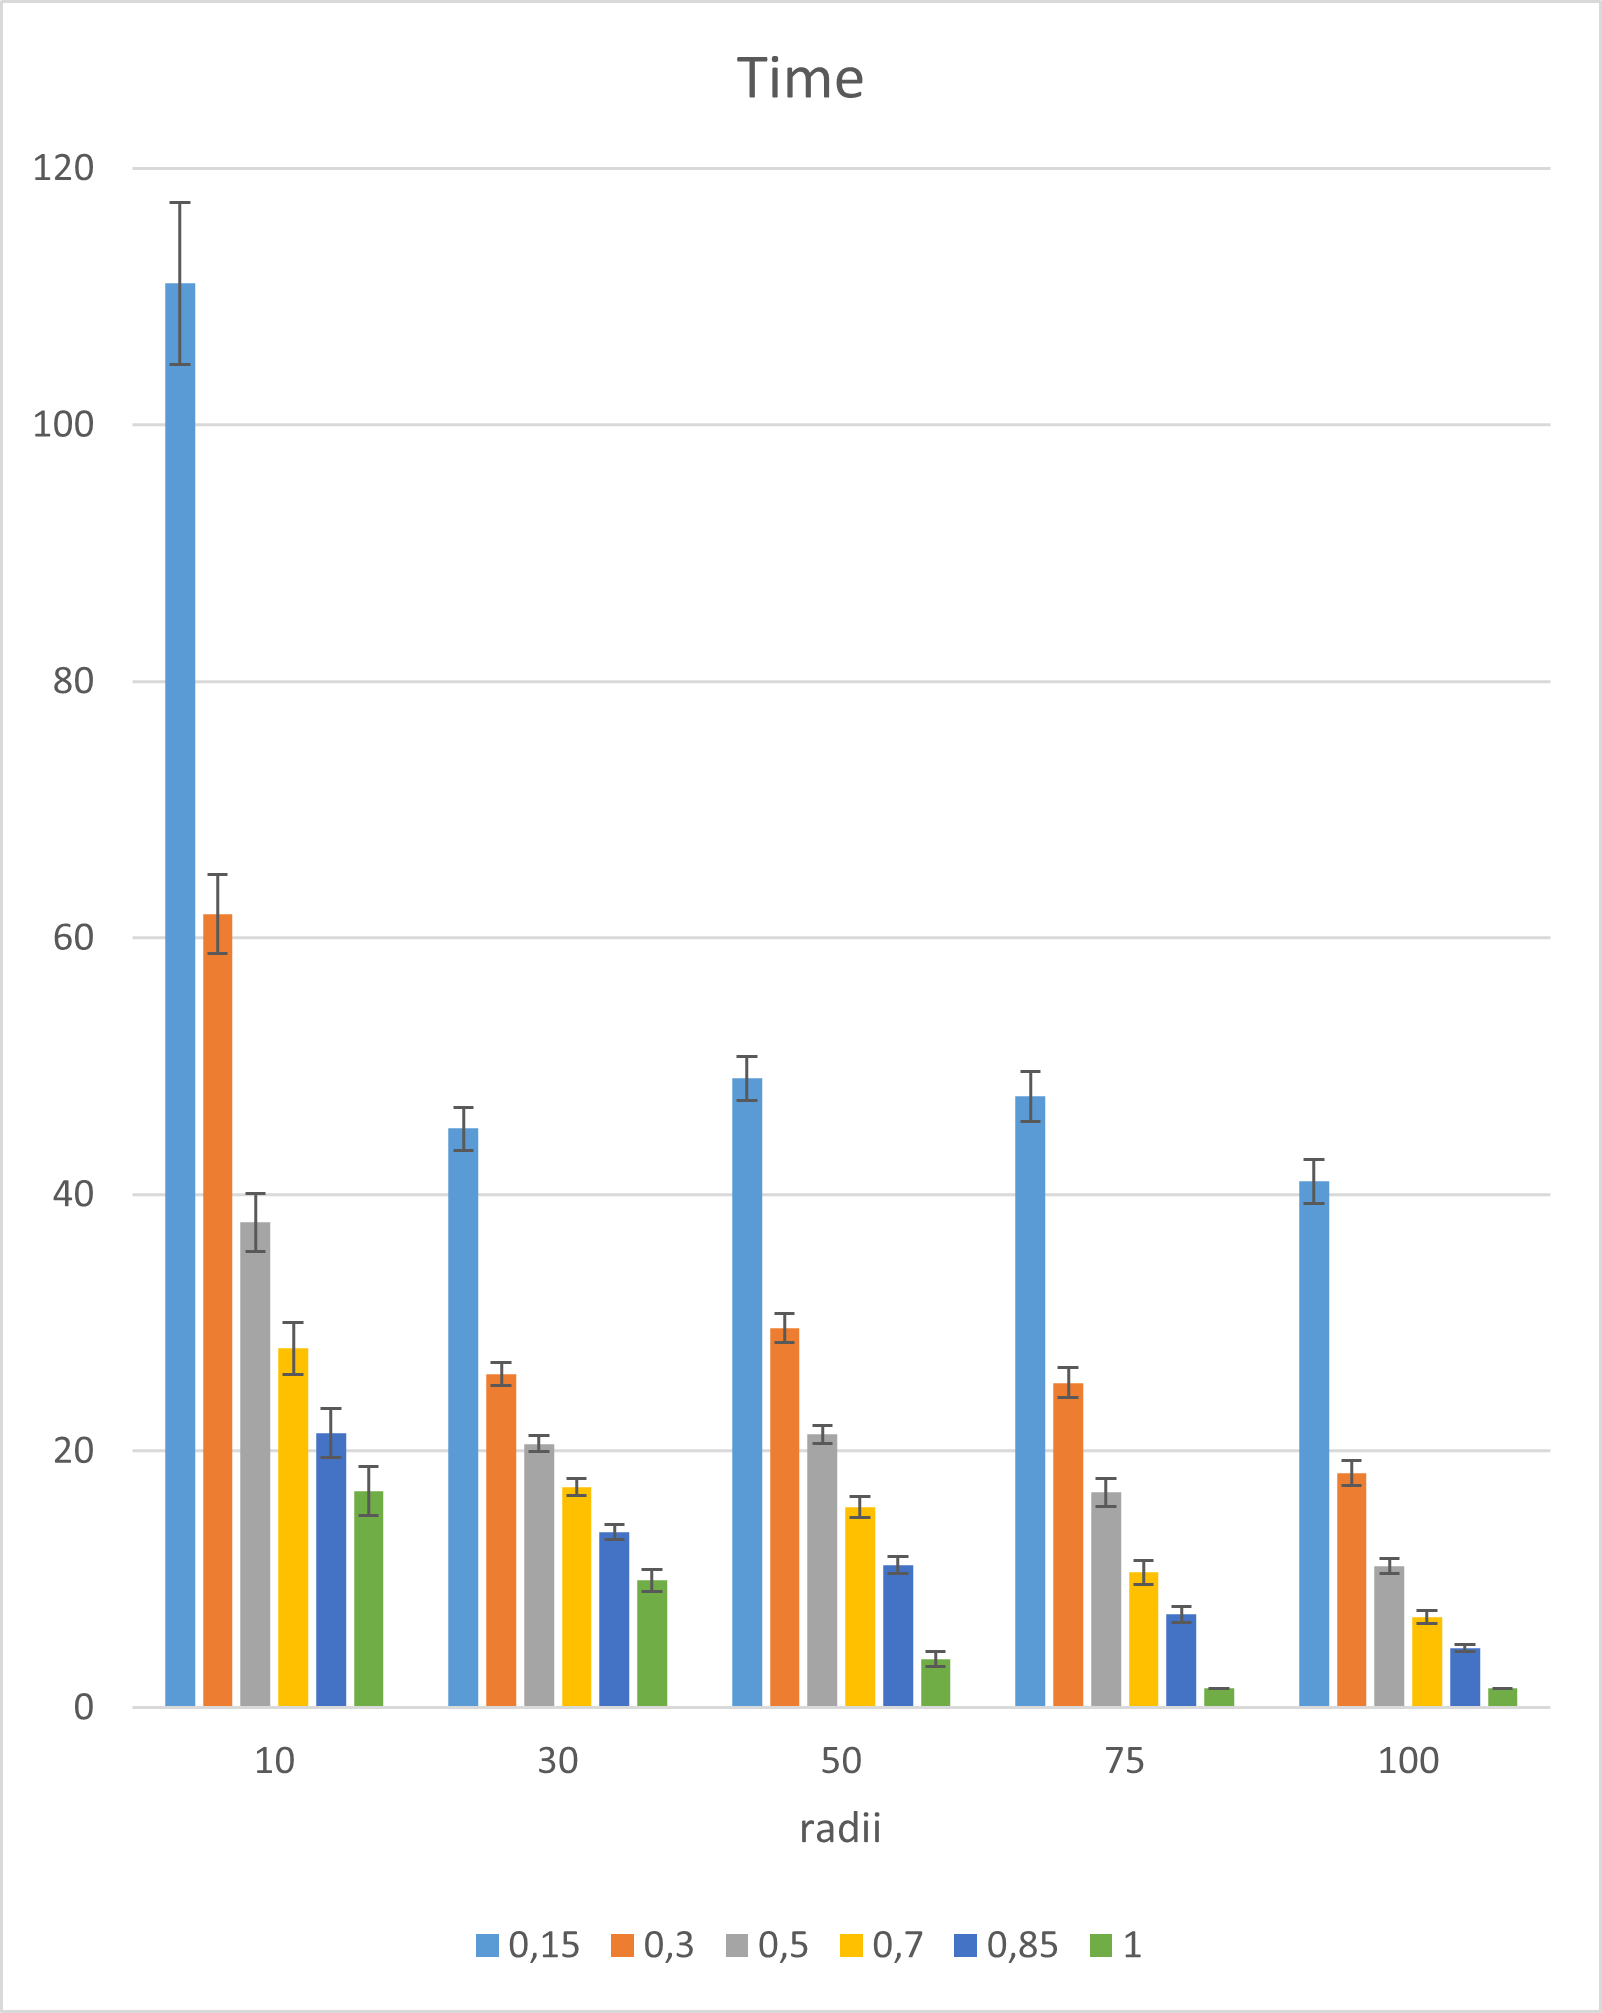
\includegraphics[width=8cm]{./images/200endtimeCI.png}}}
    \caption{Column graph with 90\% CI}
    \label{fig:200-90CI}
\end{figure}



Since the mean does not give enough information about the index variation, we decide to calculate the standard deviation as well.


\begin{table}[H]
\centering
\begin{tabular}{|c|r|r|r|r|r|}
\hline
 & \multicolumn{1}{c|}{\textbf{r=10}} & \multicolumn{1}{c|}{\textbf{r=30}} & \multicolumn{1}{c|}{\textbf{r=50}} & \multicolumn{1}{c|}{\textbf{r=75}} & \multicolumn{1}{c|}{\textbf{r=100}} \\ \hline
\textbf{p=0.15} & 0,1601 & 0 & 0 & 0 & 0 \\ \hline
\textbf{p=0.3} & 0,1215 & 0,0028 & 0,0189 & 0,0000 & 0,0044 \\ \hline
\textbf{p=0.5} & 0,2110 & 0,0069 & 0,0454 & 0,0286 & 0,0162 \\ \hline
\textbf{p=0.7} & 0,2424 & 0,0244 & 0,0665 & 0,0923 & 0,0227 \\ \hline
\textbf{p=0.85} & 0,2681 & 0,0609 & 0,1141 & 0,1120 & 0,0348 \\ \hline
\textbf{p=1} & 0,2780 & 0,1413 & 0,1709 & 0,1245 & 0,0383 \\ \hline
\end{tabular}
\caption{Standard deviation of the coverage percentage}
\label{tab:std-coverage-percentage}
\end{table}

In this way we exclude the configurations whose difference between mean and standard deviation is less than 90\%. We are interested in configurations that have a satisfactory coverage percentage, as these configurations model a reliable system.

\begin{table}[H]
\centering
\begin{tabular}{|c|c|c|c|c|c|}
\hline
 & \textbf{r=10} & \textbf{r=30} & \textbf{r=50} & \textbf{r=75} & \textbf{r=100} \\ \hline
\textbf{p=0.15} & 0,7472 & \cellcolor[HTML]{92D050}1 & \cellcolor[HTML]{92D050}1 & \cellcolor[HTML]{92D050}1 & \cellcolor[HTML]{92D050}1 \\ \hline
\textbf{p=0.3} & 0,7723 & \cellcolor[HTML]{92D050}0,9964 & \cellcolor[HTML]{92D050}0,9767 & \cellcolor[HTML]{92D050}1 & \cellcolor[HTML]{92D050}0,9949 \\ \hline
\textbf{p=0.5} & 0,5881 & \cellcolor[HTML]{92D050}0,9874 & \cellcolor[HTML]{92D050}0,9426 & \cellcolor[HTML]{92D050}0,9604 & \cellcolor[HTML]{92D050}0,9797 \\ \hline
\textbf{p=0.7} & 0,4680 & \cellcolor[HTML]{92D050}0,9555 & 0,8981 & 0,8449 & \cellcolor[HTML]{92D050}0,9676 \\ \hline
\textbf{p=0.85} & 0,3049 & 0,8813 & 0,7880 & 0,8064 & \cellcolor[HTML]{92D050}0,9449 \\ \hline
\textbf{p=1} & 0,1974 & 0,6778 & 0,5003 & 0,6385 & \cellcolor[HTML]{92D050}0,9289 \\ \hline
\end{tabular}
\caption{Runs that we decide to analyze}
\label{tab:run-to-analyze}
\end{table}

\fi

\subsection{Performance indexes} \label{200Index}
After selecting the runs to be analysed, we choose to plot the most interesting performance indicators such as: the coverage percentage (Figure \ref{fig:coverage-percentage}), the completion time (Figure \ref{fig:coverage-time200}) and the mean percentage of collisions for each time-slot (Figure \ref{fig:mean-collision-rate200}). For symmetry, the graphs also show configurations, such as the one with probability 0.7 and radius 75, even if they  should not be considered according to the previously  set standards.

\begin{figure}[h!]
\centering
    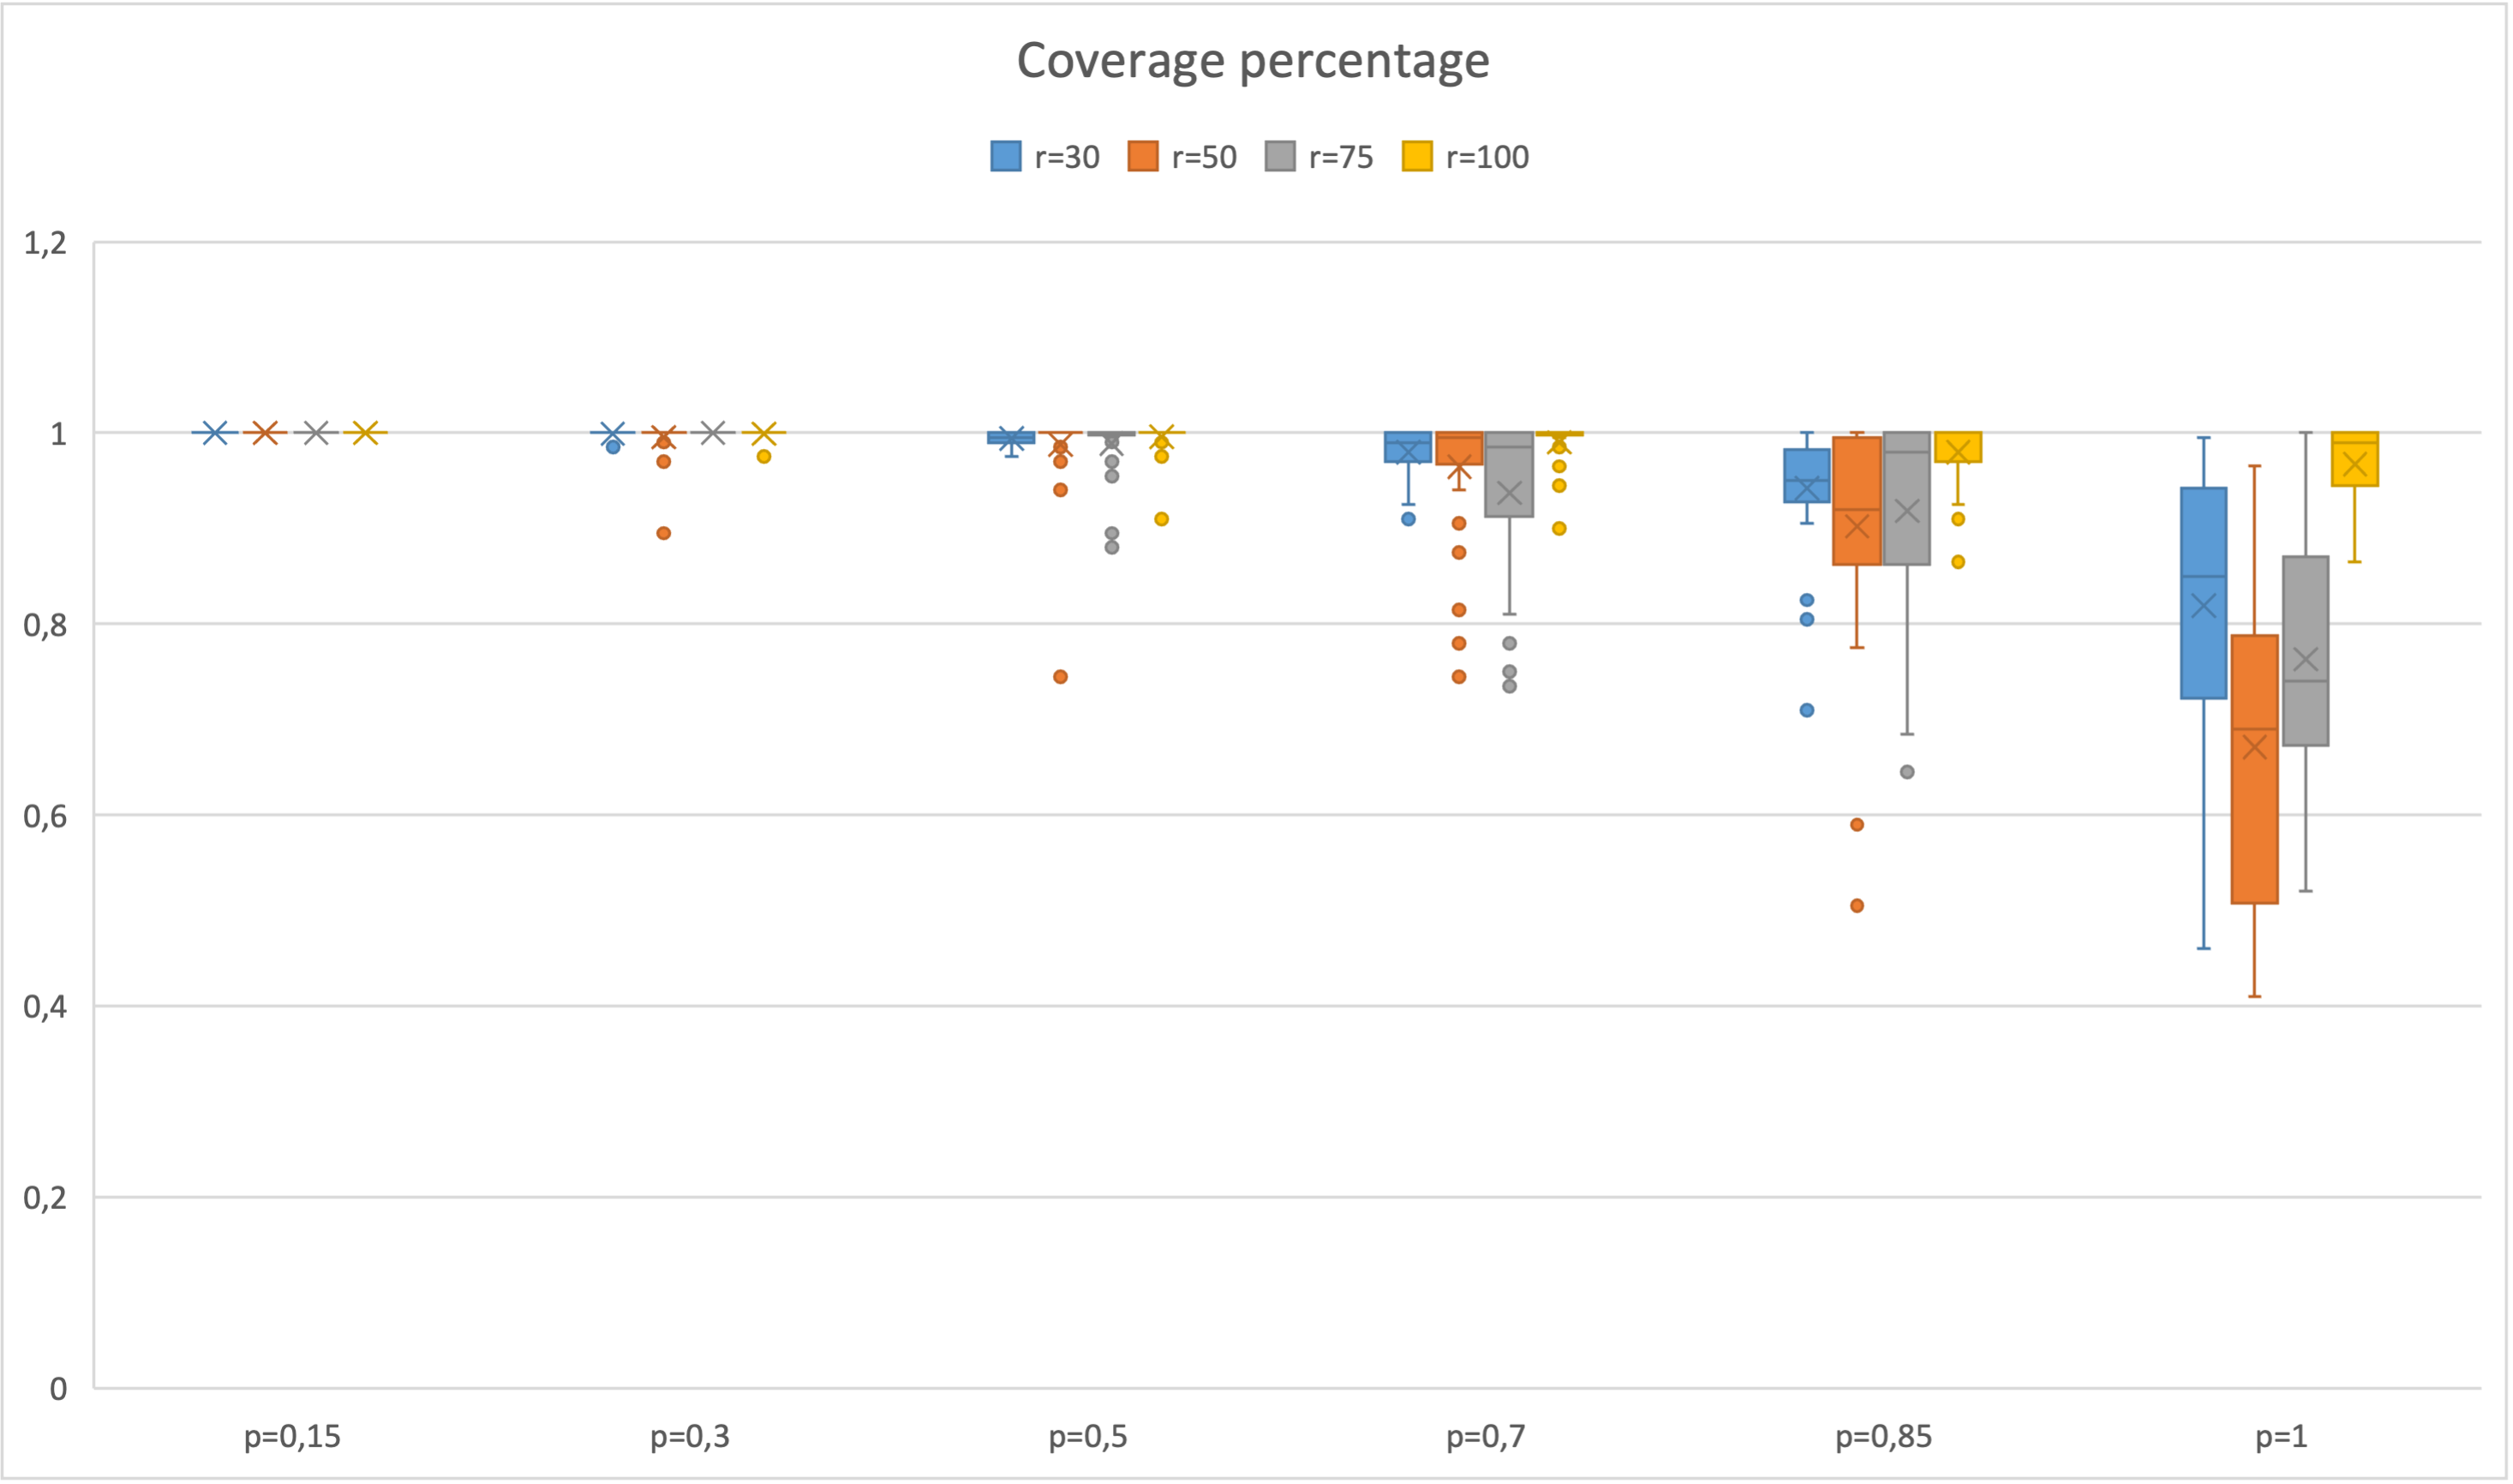
\includegraphics[width= 1\textwidth]{./images/Rate200Boxplot.png}
    \caption{Coverage percentage}
    \label{fig:coverage-percentage}
\end{figure}


\begin{figure}[h!]
\centering
    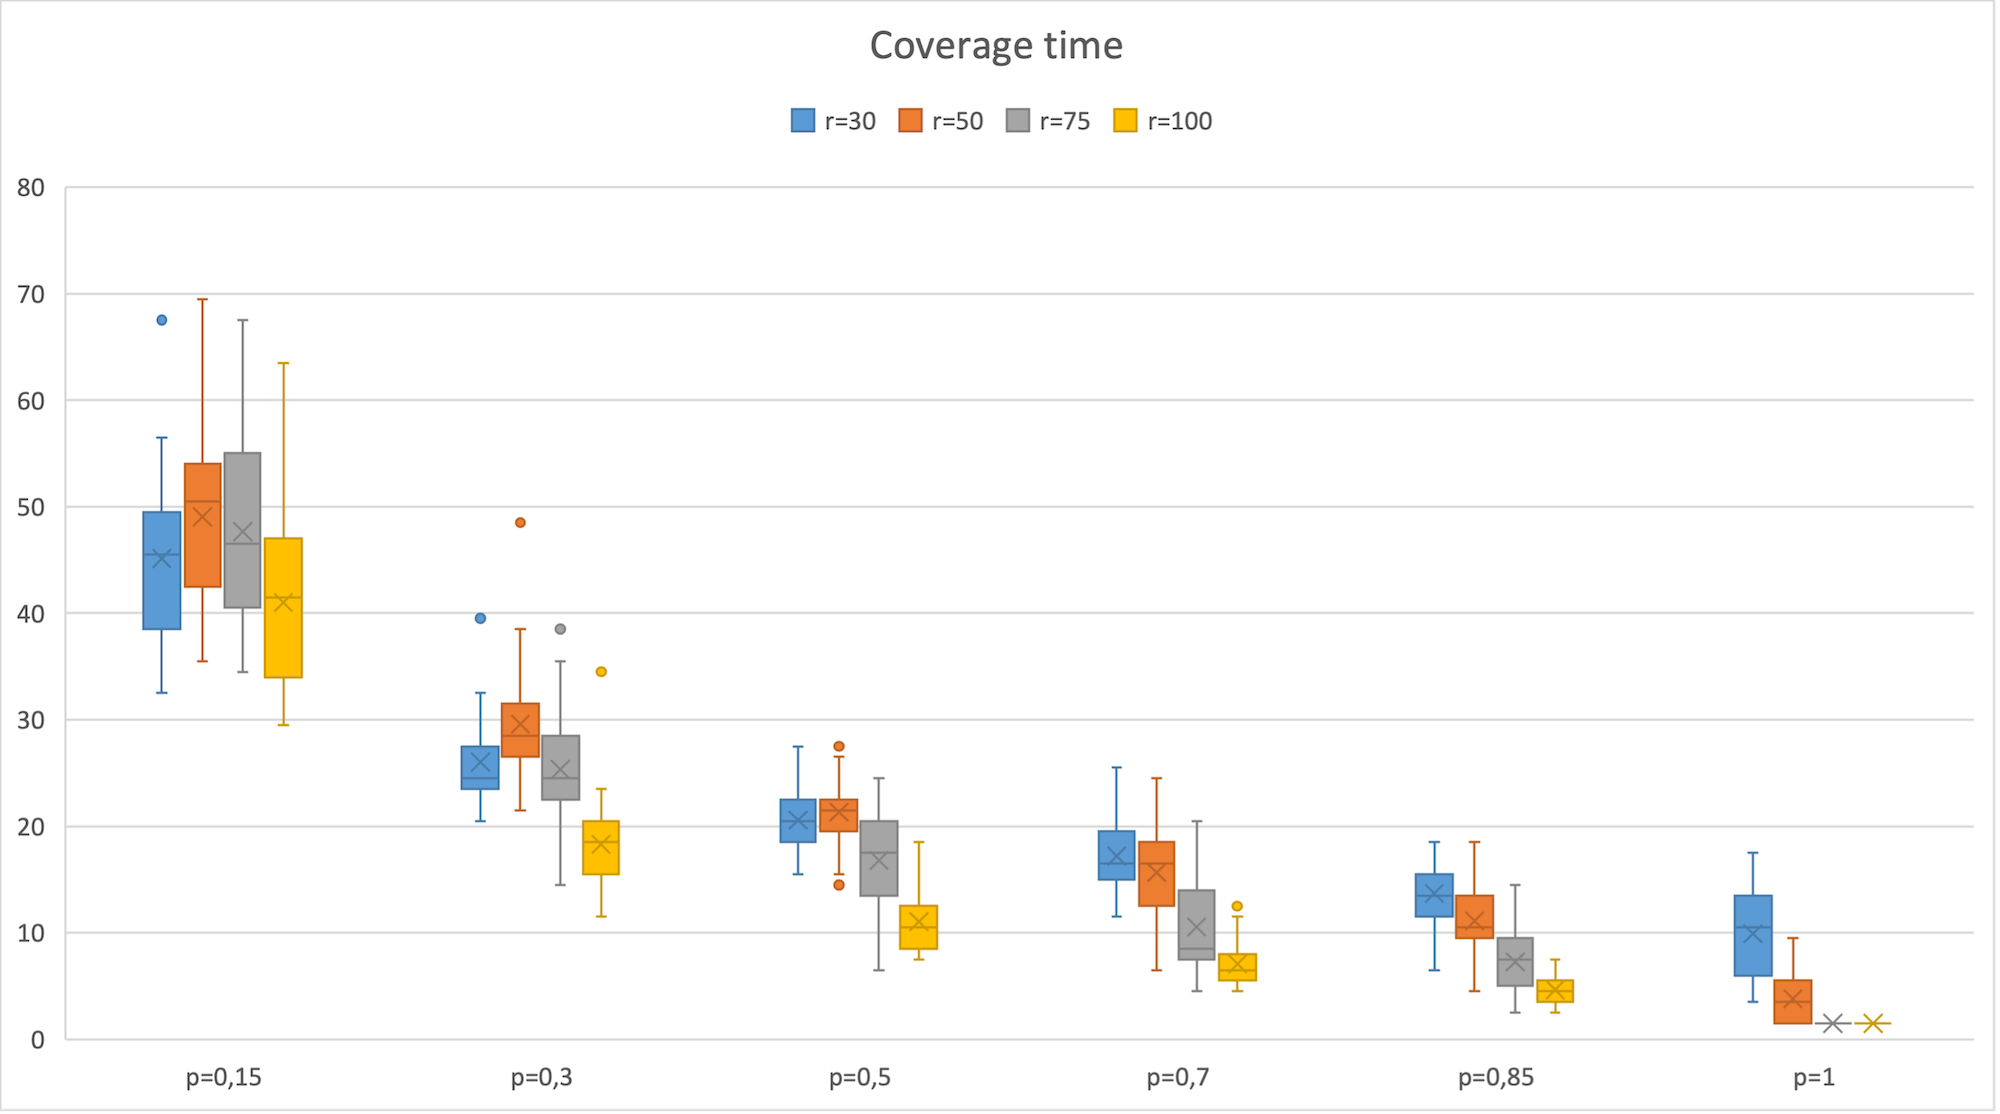
\includegraphics[width= 1\textwidth]{./images/Time200Boxplot.png}
    \caption{Coverage time}
    \label{fig:coverage-time200}
\end{figure}

\clearpage 

\begin{figure}[h!]
\centering
    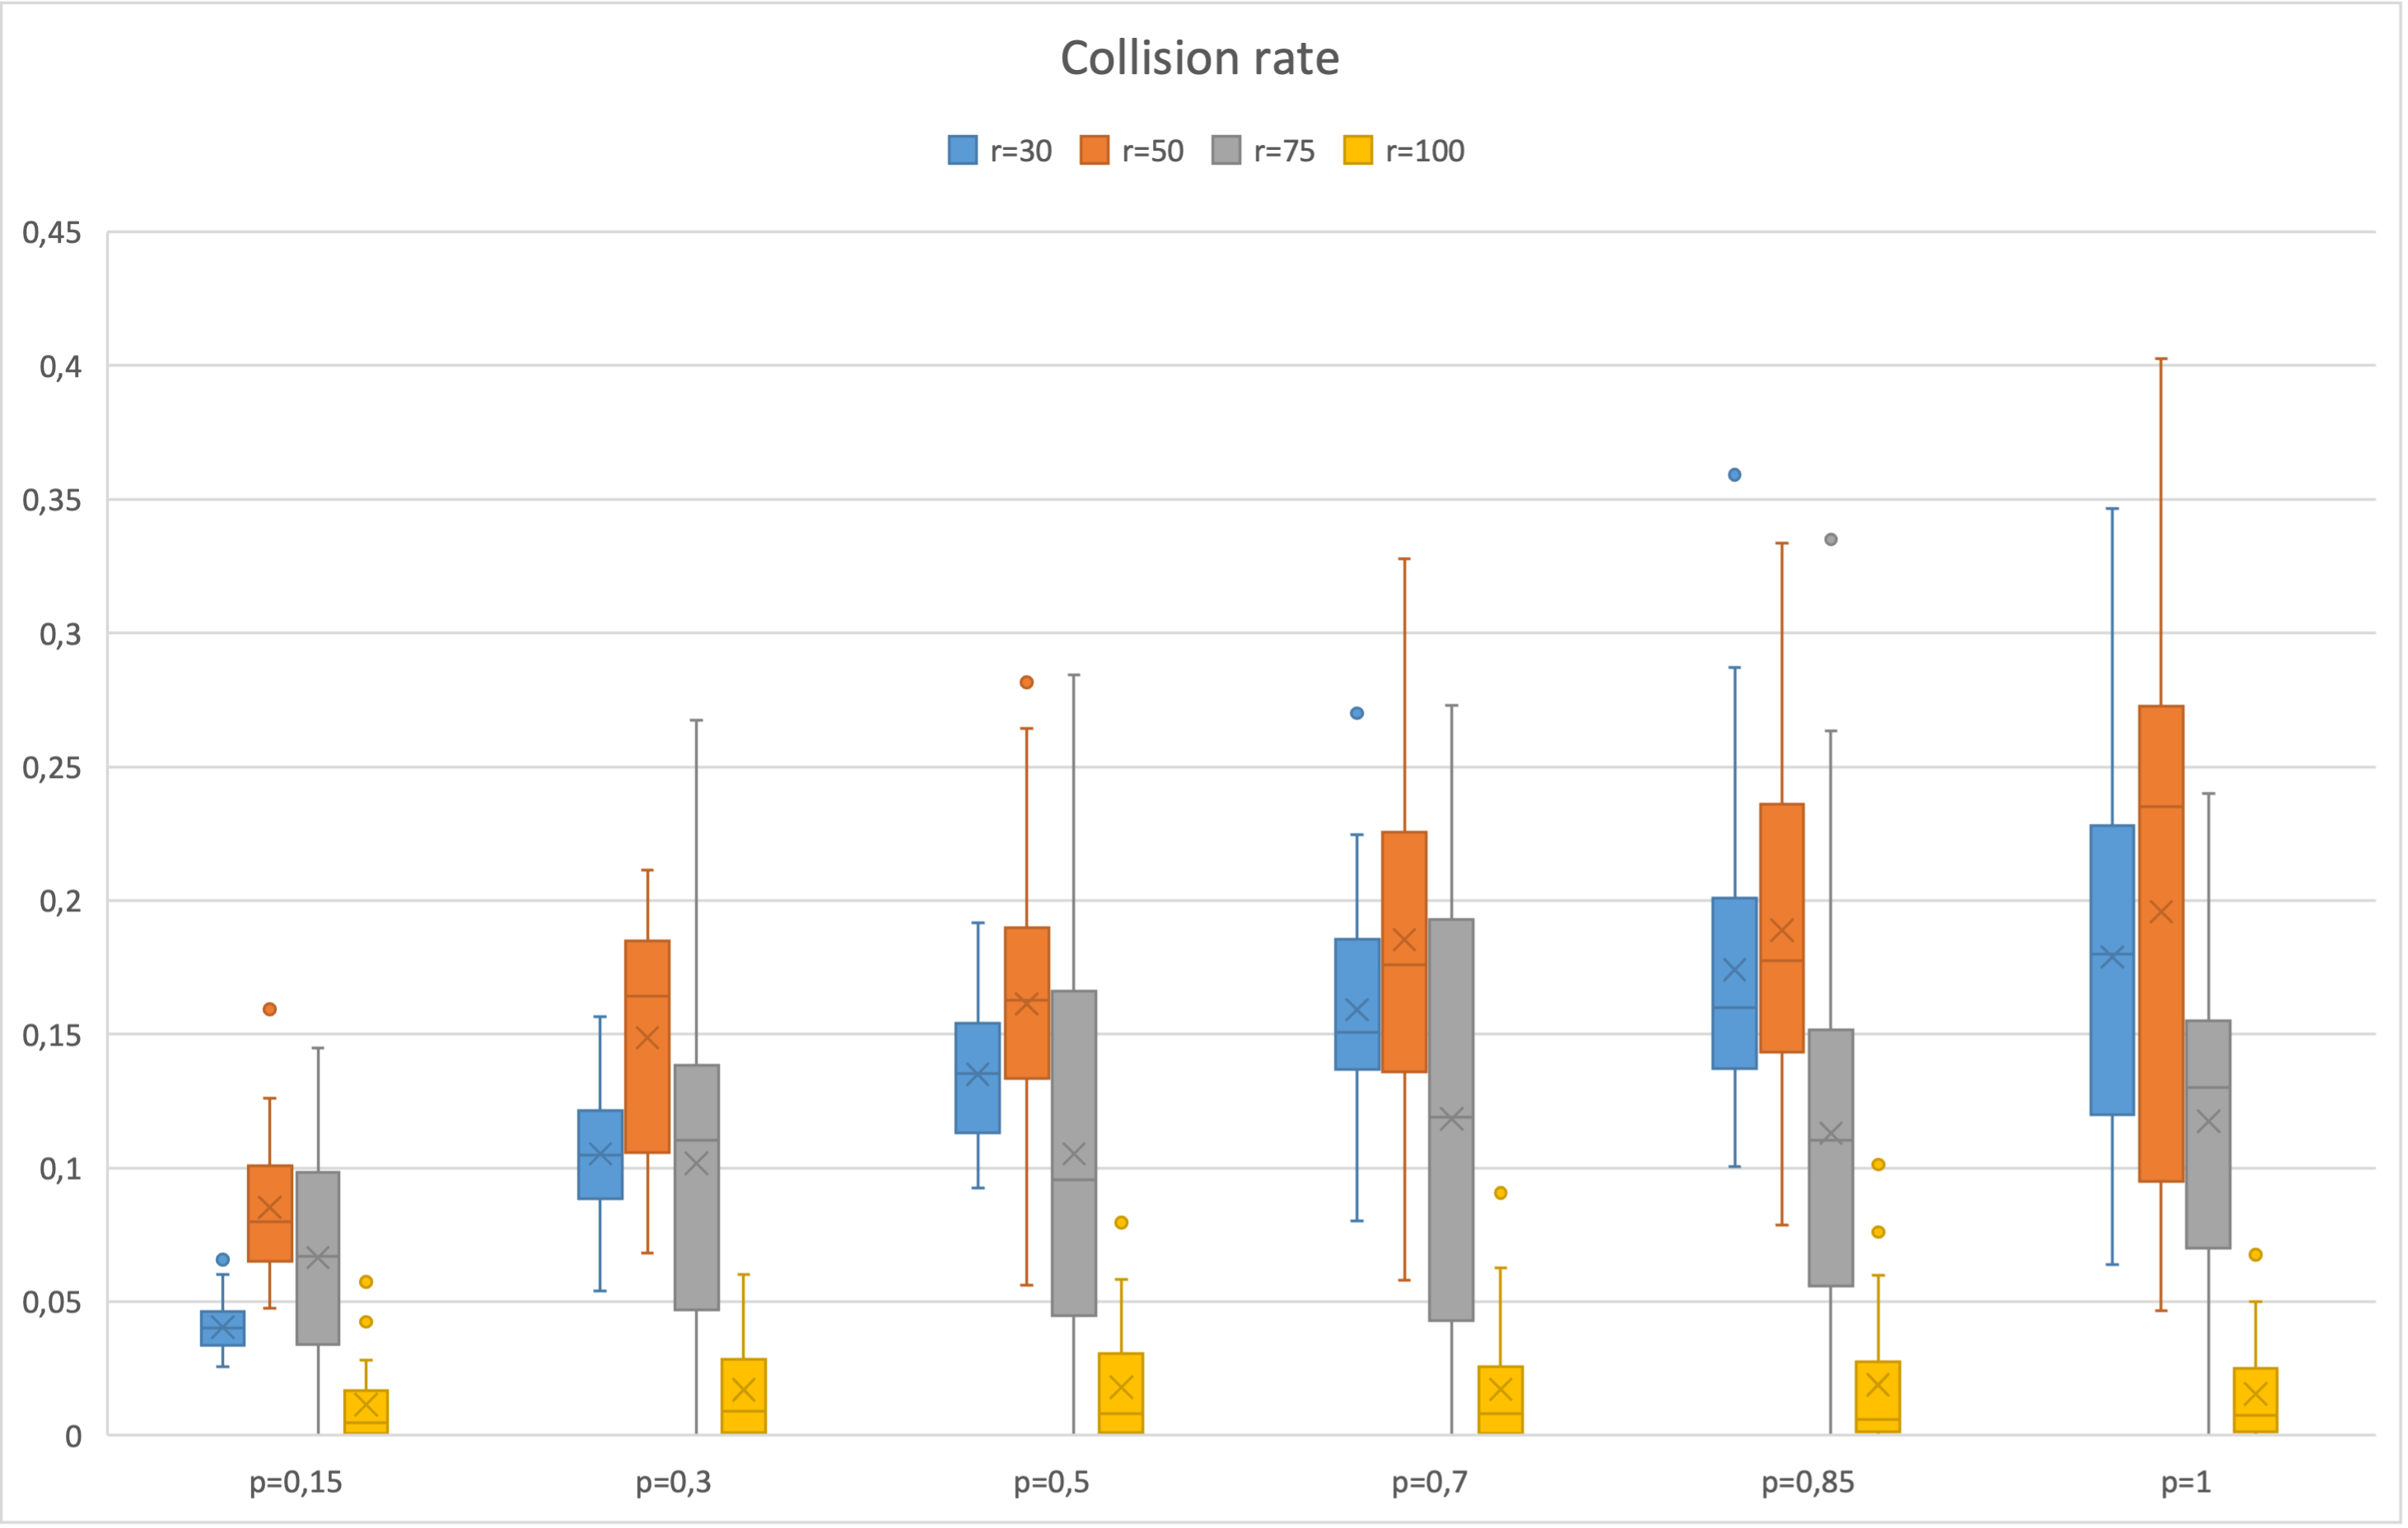
\includegraphics[width= 1\textwidth]{./images/Collision200Boxplot.png}
    \caption{Mean collision percentage}
    \label{fig:mean-collision-rate200}
\end{figure}

\noindent Looking at coverage percentage graph (Fig. \ref{fig:coverage-percentage}), it can be seen that increasing the probability does not give better coverage in most cases, as one would expect. In fact, it should be emphasized that as the probability increases, collisions also tend to increase accordingly. As imagined, the coverage time (Fig. \ref{fig:coverage-time200}) decreases as the probability increases, as a higher probability translates into more nodes that can send the infection message. Regarding the collision index (Fig \ref{fig:mean-collision-rate200}), the average values were obtained for each repetition. For this index, as expected, there is an increasing trend with the growth of probability which implies that more nodes can transmit the message in the same time-slot. It also should be noted that the cases with 75 and 100 radii do not follow the highlighted patters: the reason why is because, as the radius and the probability increase, the possibility of having many nodes reached by the infection message in the first instant is high.
\clearpage 

\subsection{Hierarchy of priorities}
Thinking of a real system we have elaborated a hierarchy of priorities to try to understand which system was the most adherent to these characteristics:

\begin{enumerate}
\item High coverage percentage
\item Minimum coverage time
\item Minimum collision percentage
\end{enumerate}

Considering runs of interest, shown in the graph \ref{fig:CoveragePercentageCI}, we filter only those with a confidence interval on the mean above the threshold.
We can rank them based on the coverage time, using Figure \ref{fig:coverage-time200} and we see that an increase in probability is clearly beneficial for a system speed-up although with a diminishing return. We can observe that the confidence interval for $p=0.3$, $r=75$ collapses to the mean value, same as almost every run with $p=0.15$ and thus given that it has the smallest coverage time between those, it is chosen as the best configuration for the previously explained metrics.

\subsection{Time evolution}\label{time-evolution}
Thanks to the data collected, we have the state of the system for each instant of time, and we are able to analyze the temporal evolution of the system. Considering the case with 200 nodes, we examine all four combinations of radius $(10-75)$ and probability $(0.15-0.85)$, plus the special configuration $p=0.30$ and $r=75$. 
Figure \ref{fig:done-status} is plotted on a linear time scale and shows the relative speed of completion for the different configuration. In particular, it is evident the negative impact given by a small probability of transmission, especially if coupled with a small radius. 
Unfortunately, this figure doesn't show confidence intervals, as they would clutter the graph too much, particularly in the most critical initial instants. 
Figure \ref{fig:done-status-log} tries to fix this problem by employing a logarithmic scale on the time axis. This allows us to better define differences between configurations, as the colored areas represent a 90\% confidence interval. It is clear that the special configuration $p=0.30$ and $r=75$ is the fastest one between those that reach a complete coverage. 
Increasing the probability makes the system faster given that we increase the radius too: this is the difference between the configuration $p=0.85$ $r=75$, which is the fastest to reach an almost $90\%$ coverage with a $90\%$ confidence level, and the configuration $p=0.85$ $r=10$, which has a higher chance of representing an unconnected graph. 
Finally, if the problem imposes a small radius, it is clear that drastically reducing the probability (configuration $p=0.15$ $r=10$) guarantees a higher final coverage in regards of other runs with higher probability (configuration $p=0.85$ $r=10$), as we get much fewer collisions. Obviously we must accept the fact that this implies a much longer wait before reaching the final state.
%which is the preferred one, considering the priorities previously considered. Indeed, we can 
\begin{figure}[H]
\centering
    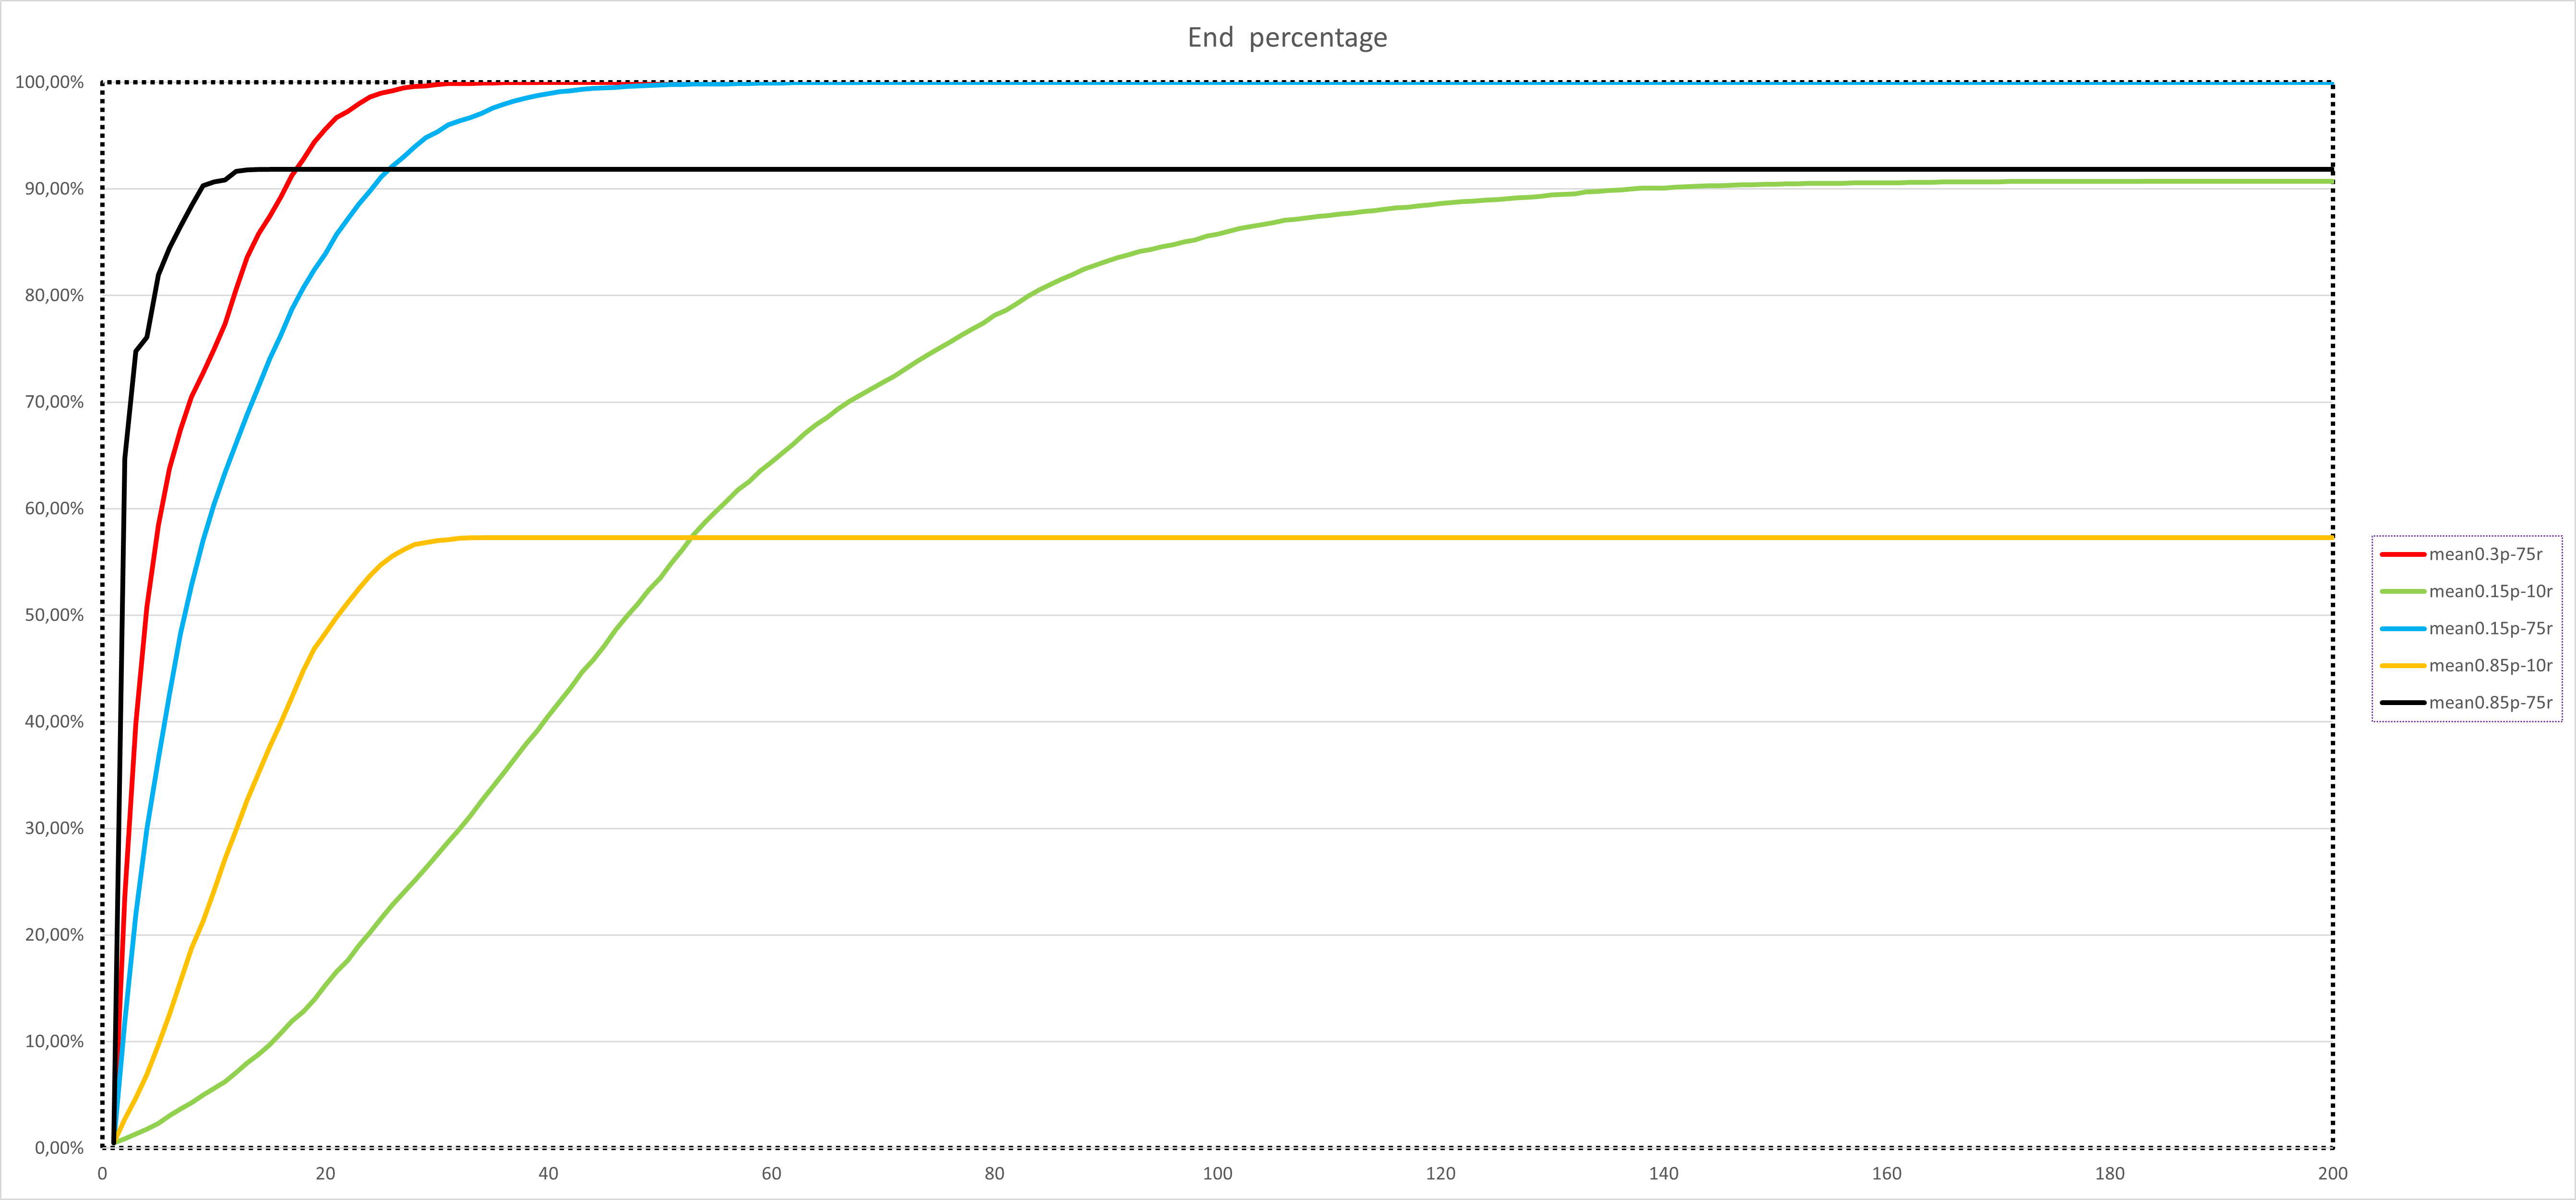
\includegraphics[width= 1\textwidth]{./images/temporalDone.png}
    \caption{Mean done status}
    \label{fig:done-status}
\end{figure}
\begin{figure}[H]
\centering
    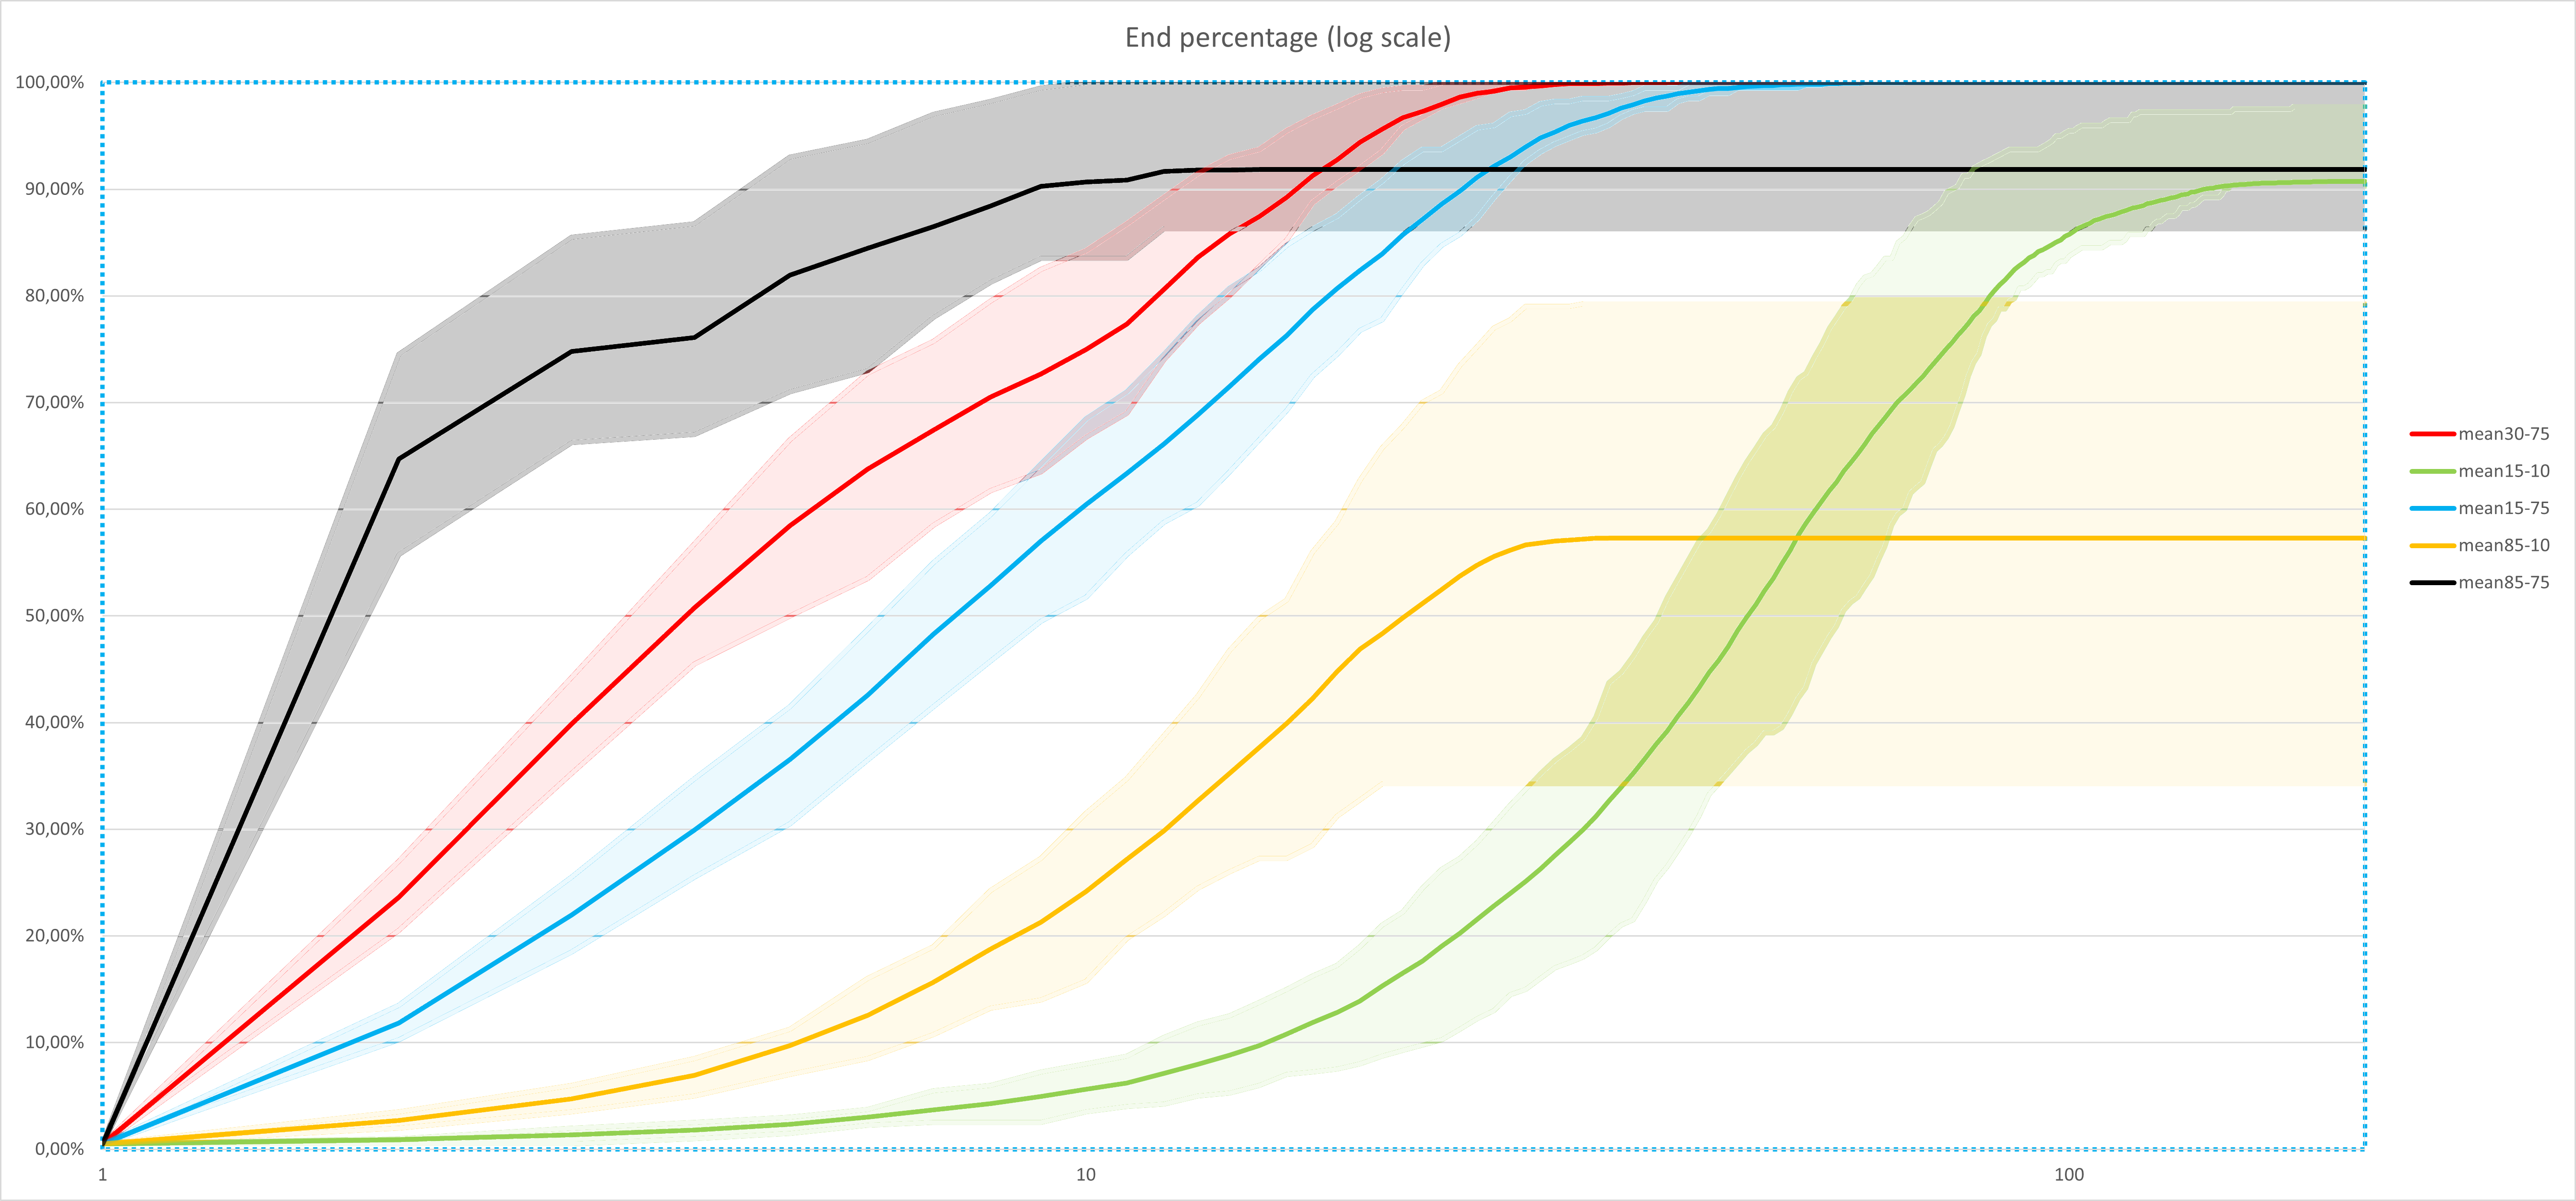
\includegraphics[width= 1\textwidth]{./images/temporalDoneLog.png}
    \caption{Done status on a logarithmic scale with 90\% CI}
    \label{fig:done-status-log}
\end{figure}

\subsection{Factorial Analysis of ending time and ending coverage}

We compute a $2^k$ factorial analysis to highlight the influence of radius $r$ and probability $p$ on two of our performance indexes, fitting the output variable to a bi-dimensional nonlinear regression model in the form of 
$$
y = q_0 + q_R \cdot r + q_P \cdot p + q_{RP} \cdot r \cdot p
$$

Starting with the final node coverage, i.e. the fraction of nodes in the Done status at the end of simulation, extreme values are shown in Table \ref{tab:extreme-factors-end-coverage} and the final influence in Table \ref{tab:influence-on-end-coverage}. It is important to notice that the extremes do not include a sending probability of 100\% and radius of 100 because we decide to handle these as particular configurations that serve only to show the limit cases for the system.


\begin{table}[h!]
\centering
\begin{tabular}{|cc|cc|}
\hline
\multicolumn{2}{|c|}{\multirow{2}{*}{\textbf{Coverage percentage}}} & \multicolumn{2}{c|}{\textbf{Radius}} \\ \cline{3-4} 
\multicolumn{2}{|c|}{} & \multicolumn{1}{c|}{\textbf{10}} & \textbf{75} \\ \hline
\multicolumn{1}{|c|}{\multirow{2}{*}{\textbf{Probability}}} & \textbf{15} & \multicolumn{1}{c|}{0,9073} & 1 \\ \cline{2-4} 
\multicolumn{1}{|c|}{} & \textbf{85} & \multicolumn{1}{c|}{0,5730} & 0,9183 \\ \hline
\end{tabular}
\caption{Extreme factor levels for ending coverage}
\label{tab:extreme-factors-end-coverage}
\end{table}

\begin{table}[H]
\centering
\begin{tabular}{c|c|c|c|c|cc}
\cline{2-7}
 & \textbf{I} & \textbf{Probability} & \textbf{Radius} & \textbf{Combined} & \multicolumn{1}{c|}{\textbf{Cov. Perc}} & \multicolumn{1}{c|}{\textbf{SD\_i}} \\ \cline{2-7} 
 & 1 & -1 & -1 & 1 & \multicolumn{1}{c|}{0,9073} & \multicolumn{1}{c|}{0,0033} \\ \cline{2-7} 
 & 1 & 1 & -1 & -1 & \multicolumn{1}{c|}{0,5730} & \multicolumn{1}{c|}{0,0765} \\ \cline{2-7} 
 & 1 & -1 & 1 & -1 & \multicolumn{1}{c|}{1,0000} & \multicolumn{1}{c|}{0,0226} \\ \cline{2-7} 
 & 1 & 1 & 1 & 1 & \multicolumn{1}{c|}{0,9183} & \multicolumn{1}{c|}{0,0047} \\ \hline
\multicolumn{1}{|c|}{\textbf{4q}} & 3,3986 & -0,4159 & 0,4380 & 0,2526 & \multicolumn{1}{c|}{Total} & \multicolumn{1}{c|}{0,1072} \\ \hline
\multicolumn{1}{|c|}{\textbf{q}} & 0,8497 & -0,1040 & 0,1095 & 0,0631 &  &  \\ \cline{1-5}
\multicolumn{1}{|c|}{\textbf{4 q\textasciicircum{}2}} &  & 0,0432 & 0,0480 & 0,0159 &  &  \\ \cline{1-5}
\multicolumn{1}{|c|}{\textbf{Influence}} &  & 0,4036 & 0,4476 & 0,1488 &  &  \\ \cline{1-5}
\end{tabular}
\caption{Influence of factors for ending coverage}
\label{tab:influence-on-end-coverage}
\end{table}


We get a pretty balanced influence between radius and probability of about $\sim 42\%$ each, although we must notice that the term $q_P$ is negative $(-0.10)$, which implies a reduction of the final coverage with an increase in probability. Looking at Figure \ref{fig:mean-collision-rate200} we can clearly understand that this is primarily due to an increase in collisions, which naturally reflects the much lower coverage. Finally, we can assess that the interaction of both parameters is relatively small $(14\%)$, and thus we can study the system by just fixing one parameter and varying the other.

Regarding the completion time, the extreme values are shown in Table \ref{tab:extreme-factors-time-coverage} and influences in Table \ref{tab:influence-on-time-coverage}

\begin{table}[h!]
\centering
\begin{tabular}{|cc|cc|}
\hline
\multicolumn{2}{|c|}{\multirow{2}{*}{\textbf{Coverage time}}} & \multicolumn{2}{c|}{\textbf{Radius}} \\ \cline{3-4} 
\multicolumn{2}{|c|}{} & \multicolumn{1}{c|}{\textbf{10}} & \textbf{75} \\ \hline
\multicolumn{1}{|c|}{\multirow{2}{*}{\textbf{Probability}}} & \textbf{15} & \multicolumn{1}{c|}{111,0152} & 47,6515 \\ \cline{2-4} 
\multicolumn{1}{|c|}{} & \textbf{85} & \multicolumn{1}{c|}{21,4091} & 7,2576 \\ \hline
\end{tabular}
\caption{Extreme level of factors for time coverage}
\label{tab:extreme-factors-time-coverage}
\end{table}

\begin{table}[H]
\centering
\begin{tabular}{c|c|c|c|c|cc}
\cline{2-7}
 & \textbf{I} & \textbf{Probability} & \textbf{Radius} & \textbf{Combined} & \multicolumn{1}{c|}{\textbf{Cov. time}} & \multicolumn{1}{c|}{\textbf{SD\_i}} \\ \cline{2-7} 
 & 1 & -1 & -1 & 1 & \multicolumn{1}{c|}{111,0152} & \multicolumn{1}{c|}{4119,3058} \\ \cline{2-7} 
 & 1 & 1 & -1 & -1 & \multicolumn{1}{c|}{21,4091} & \multicolumn{1}{c|}{646,3921} \\ \cline{2-7} 
 & 1 & -1 & 1 & -1 & \multicolumn{1}{c|}{47,6515} & \multicolumn{1}{c|}{0,6694} \\ \cline{2-7} 
 & 1 & 1 & 1 & 1 & \multicolumn{1}{c|}{7,2576} & \multicolumn{1}{c|}{1566,2406} \\ \hline
\multicolumn{1}{|c|}{\textbf{4q}} & 187,3333 & -130,0000 & -77,5152 & 49,2121 & \multicolumn{1}{c|}{Total} & \multicolumn{1}{c|}{6332,6079} \\ \hline
\multicolumn{1}{|c|}{\textbf{q}} & 46,8333 & -32,5000 & -19,3788 & 12,3030 &  &  \\ \cline{1-5}
\multicolumn{1}{|c|}{\textbf{4 q\textasciicircum{}2}} &  & 4225,0000 & 1502,1497 & 605,4582 &  &  \\ \cline{1-5}
\multicolumn{1}{|c|}{\textbf{Influence}} &  & 0,6672 & 0,2372 & 0,0956 &  &  \\ \cline{1-5}
\end{tabular}
\caption{Influence of factors for time coverage}
\label{tab:influence-on-time-coverage}
\end{table}

It is clear that having both negative coefficients ($q_P = -32.50$ and $q_R = -19.38$) is beneficial for a faster system termination (lower is better). The probability is also $\sim\times 3$ more effective at reducing the completion time, which is also stated by Figure \ref{fig:coverage-time200} and is in line with what is expected: even if it means having more collisions, having a higher probability reduces the time a node waits in the Ready status. Again, the interaction of both parameters is negligible and allows us to study the effect of each parameter separately.
